\documentclass[main.tex]{subfiles}
\begin{document}

\section{Heaviside Step Function}

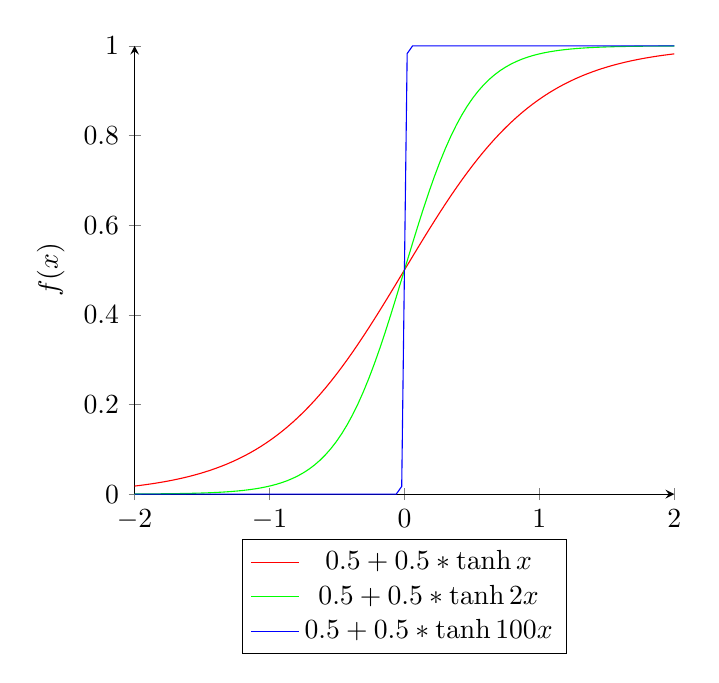
\begin{tikzpicture}
\begin{axis}[
    axis lines = left,
    xlabel = $x$,
    ylabel = {$f(x)$},
    legend style={at={(0.5,-0.1)},anchor=north}
]

\addplot [
    domain=-2:2, 
    samples=100, 
    color=red,
]
{0.5 + 0.5*tanh(x)};
\addlegendentry{$0.5 + 0.5*\tanh{x}$}

\addplot [
    domain=-2:2, 
    samples=100, 
    color=green,
    ]
    {0.5 + 0.5*tanh(2*x)};
\addlegendentry{$0.5 + 0.5*\tanh{2x}$}

\addplot [
    domain=-2:2, 
    samples=100, 
    color=blue,
    ]
    {0.5 + 0.5*tanh(100*x)};
\addlegendentry{$0.5 + 0.5*\tanh{100x}$}

\end{axis}
\end{tikzpicture}

\par
As you can see, the higher the multiplier to $x$ the steeper the curve on the transition from $0$ to $1$.

\end{document}